\chapter{The CMS experiment}
\label{chap:detector}

\section{The LHC}
\label{sec:theLHC}

The Large Hadron Collider (LHC) \cite{theLHC} is a synchrotron accelerator
with a $27\,\kilo\metre$ circumference designed to
collide beams of protons at centre of mass energies as high as $14\,\TeV$. It is
hosted in the tunnel of the former Large Electron Positron (LEP)
\cite{LEP:1983aa} accelerator on the French-Swiss border
near Geneva and operated by the European Organisation for Nuclear Research
(CERN). As well as proton-proton collisions, the LHC also accelerates beams of
lead ions to produce both lead-lead (PbPb) and proton-lead (pPb) collisions.

Protons originate from hydrogen gas, the atoms of which are stripped of
their electrons using an electric field. The protons are then accelerated to an
energy of $50\,\MeV$ in the Linac 2 accelerator. Proton bunches are formed inside
the \ac{PSB}, increasing the energy to $1.4\,\GeV$. The \ac{PS} creates proton
beams from the bunches, increasing the energy to $26\,\GeV$. Further acceleration
in the \ac{SPS} raises the beam energy to $450\,\GeV$ before being injected into
the LHC. The LHC contains two beams circulating in opposite directions. The
design operation conditions consist of each beam containing up to 2808 bunches
spaced $25\,\ns$ apart and made up of $\mathcal{O}(10^{11})$ protons each. 
Approximately 1200 superconducting dipole magnets keep the beams circulating
before collisions. The beams collide at four points around the LHC where they
are recorded by four detectors: ALICE \cite{Aamodt:2008zz}, ATLAS
\cite{Aad:2008zzm}, CMS \cite{Chatrchyan:2008aa} and LHCb \cite{Alves:2008zz}. A
schematic of the LHC ring and the detectors is shown in figure
\ref{fig:LHCschematic}.

\begin{figure}[htbp]
   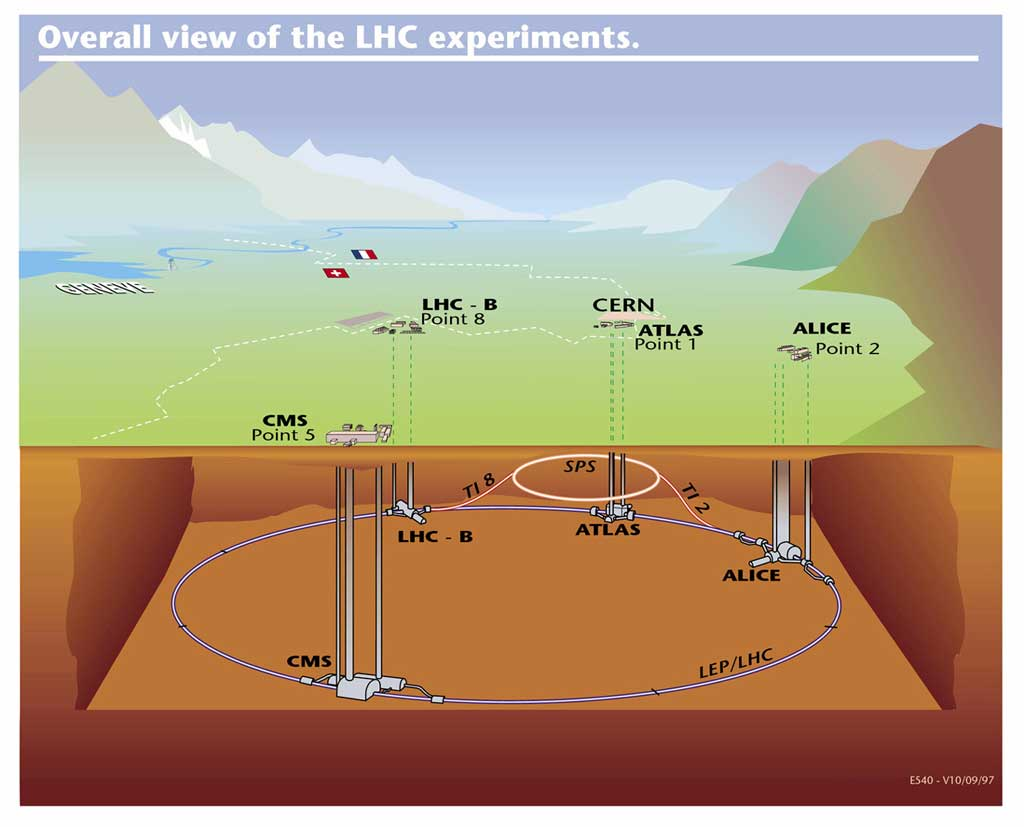
\includegraphics[width=0.7\textwidth]{plots/detector/LHC_layout_sch.jpg}
\caption{Schematic of the LHC accelerator, showing the positions of the four
large detectors.}
\label{fig:LHCschematic}
\end{figure}

The LHC was designed to study physics at the $\TeV$ scale. One of the major
goals of the ATLAS and CMS detectors is to understand the mechanism behind
electroweak symmetry breaking and search for the Higgs boson predicted by this
mechanism in the \ac{SM}. The detectors are also used in searches for \ac{BSM}
physics, with the huge acceleration power of the LHC allowing studies of 
interactions at higher energies than have ever been possible before. 

Higgs boson production occurs only rarely amongst other possible interactions from known
\ac{SM} processes. Figure~\ref{fig:LHCcrosssections} shows the cross sections of
some of these processes compared with the total proton-proton cross section. It can be
seen that \ac{SM} Higgs boson production has a cross section some $10^{9}$ times
smaller than the total proton-proton cross section. 
As such, it is necessary to collect large numbers of
collisions to ensure sufficient numbers of events containing these rare
processes. Hence the LHC operates at a high instantaneous luminosity of up to
$10^{34}\,\lumiunits$, where luminosity is given by:

\begin{equation}
L=\frac{N_{b}^{2}n_{b}f_{\text{rev}}\gamma}{4\pi\epsilon_{n}\beta^{*}}F,
\end{equation}

where $N_{b}$ is the number of protons in the bunch, $n_{b}$ is the number of
bunches, $f_\text{rev}$ is the revolution frequency, $\gamma$ is the Lorentz
factor, $\epsilon_{n}$ is the normalised emittance, $\beta^{*}$ is the beta
function at the collision point and $F$ is a reduction factor due to the
crossing angle.

\begin{figure}[htbp]
   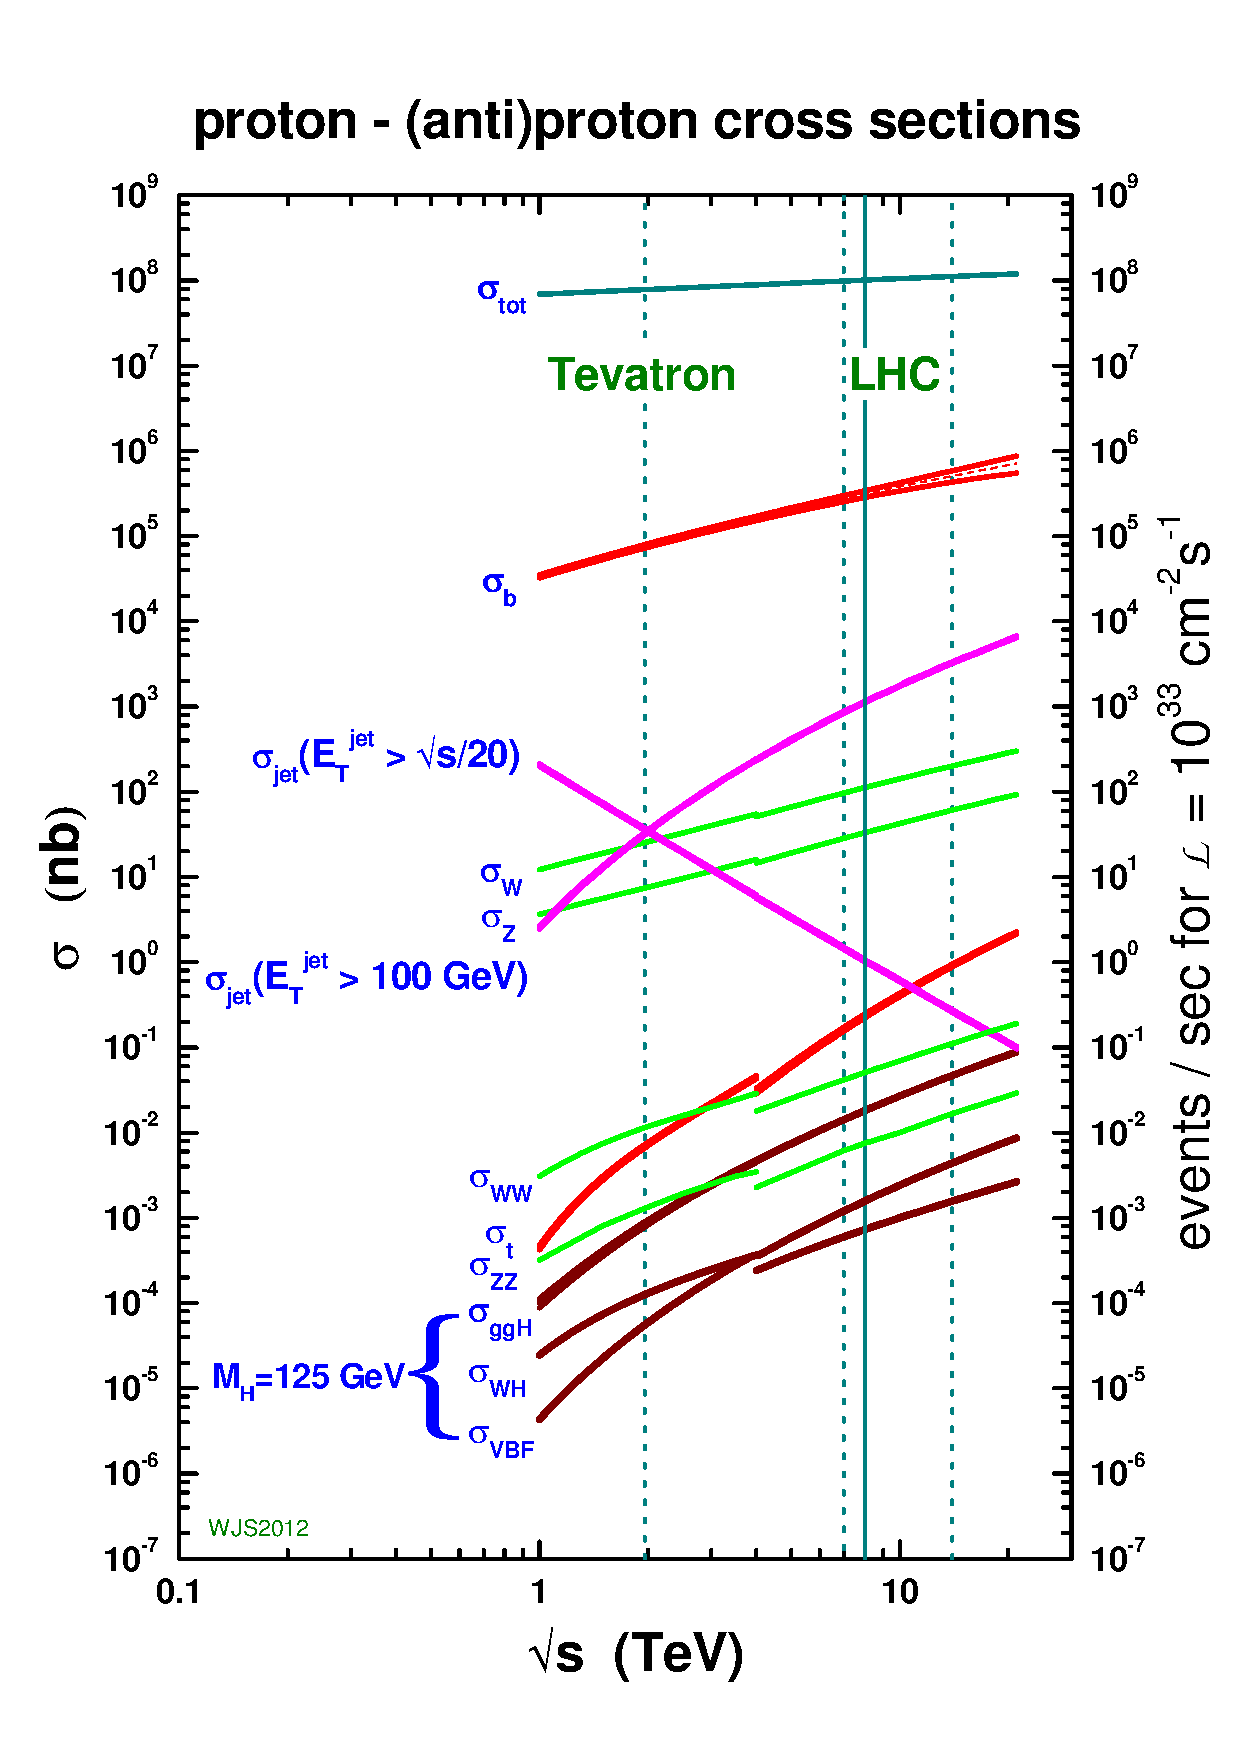
\includegraphics[width=0.6\textwidth]{plots/detector/crosssections2012_v5.pdf}
\caption[Cross sections for several processes in proton-proton or proton-anti
proton collisions, dependent on centre of mass energy.]
{Cross sections for several processes in proton-proton or proton-anti
proton collisions, dependent on centre of mass energy. Energies of the LHC at
different points in running history are highlighted, as is the energy of the
Tevatron. It can be seen that even with the high energies of the LHC, the
cross section for Higgs boson production is several orders of magnitude smaller than
the total cross section \cite{stirling:xsecs}.}
\label{fig:LHCcrosssections}
\end{figure}

The LHC began its first major physics run in May 2010 with a centre of mass
energy of $\sqrt{s} = 7\,\TeV$ and produced an integrated luminosity of
$\sim48\,\invpb$ before the winter break. It then continued at $\sqrt{s} = 7\,\TeV$
producing an integrated luminosity of $\sim6.1\,\invfb$ in 2011, before increasing to
$\sqrt{s} = 8\,\TeV$ for the 2012 run, where it provided $23.3\,\invfb$,
completing Run 1 of the LHC.
During this time the LHC operated with a bunch spacing of $50\,\ns$. 
Figure~\ref{fig:detlumi} shows the summary of the
integrated luminosity delivered to the CMS detector during Run 1 of the LHC,
which concluded in early 2013. The efficiency with which CMS took the available
data was around $91\%$ in 2011 and $93\%$ in 2012. Not all luminosity delivered by the LHC is
certified for use in physics analyses - only those events where it is known that
the whole CMS detector was operating successfully, and so the usable luminosity
was reduced to $5.1\,\invfb$ in 2011 and $19.7\,\invfb$ in 2012.
It was after the 2011 run and $\approx6\,\invfb$ of the 2012 run that the
observation of a boson consistent with the Higgs boson of the \ac{SM} was
announced in July 2012 \cite{CMSobservation125,ATLASobservation125}. 

\begin{figure}[htbp]
   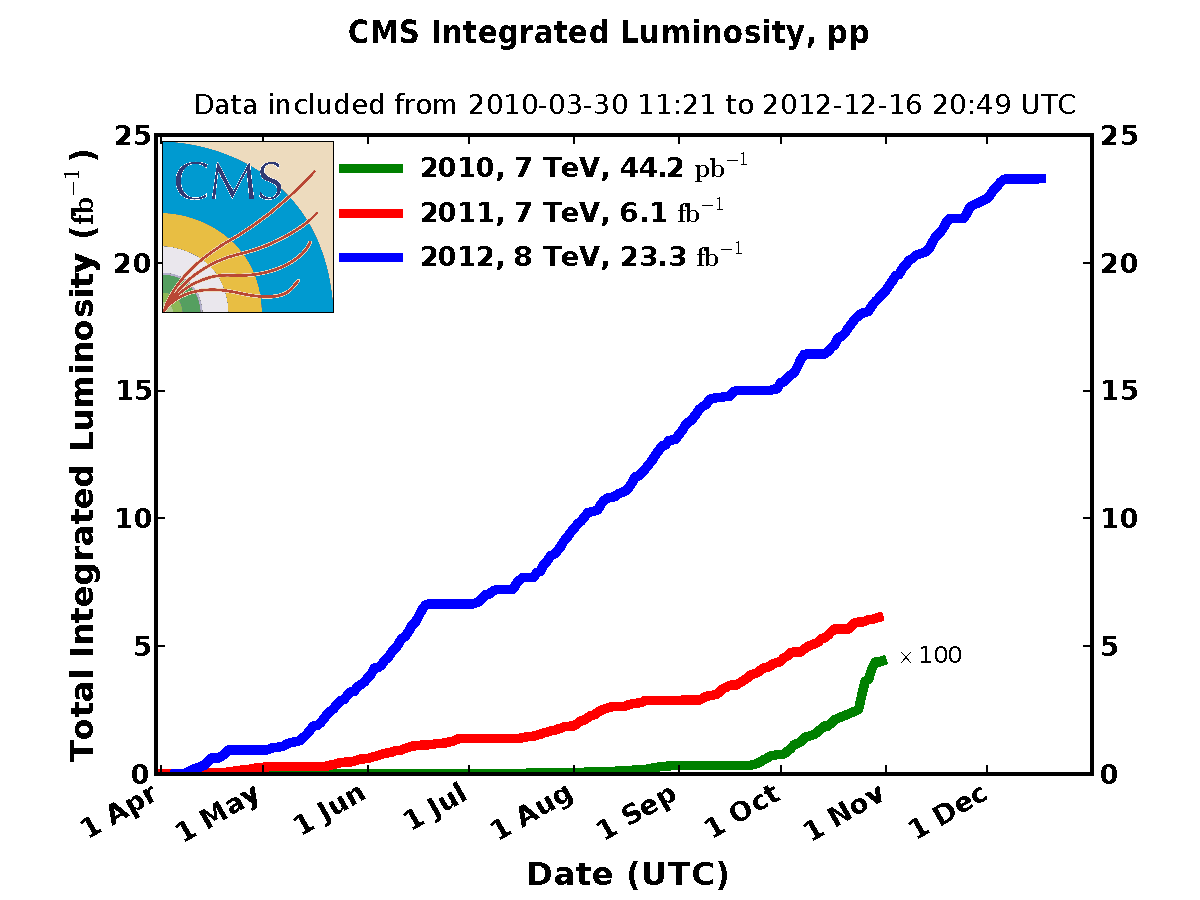
\includegraphics[width=0.7\textwidth]{plots/detector/int_lumi_cumulative_pp_2.pdf}
\caption[Illustration of the total integrated luminosity delivered to CMS during
Run 1 of the LHC.]{Illustration of the total integrated luminosity collected by
CMS during Run 1 of the LHC, separated into the 3 years of running \cite{cmslumitwiki}.}
\label{fig:detlumi}
\end{figure}

Since the LHC operates at such high luminosity, the probability of multiple
proton-proton collisions occurring in each bunch crossing is very high. Figure 
\ref{fig:PU} shows the number of interactions per bunch crossing in the
2012 dataset, where the average number was 21. The number for 2011 was slightly
lower at 9 due to the lower instantaneous luminosity. 
These additional collisions on top of the interesting hard collision
in an event are referred to as \ac{PU}.

\begin{figure}[htbp]
   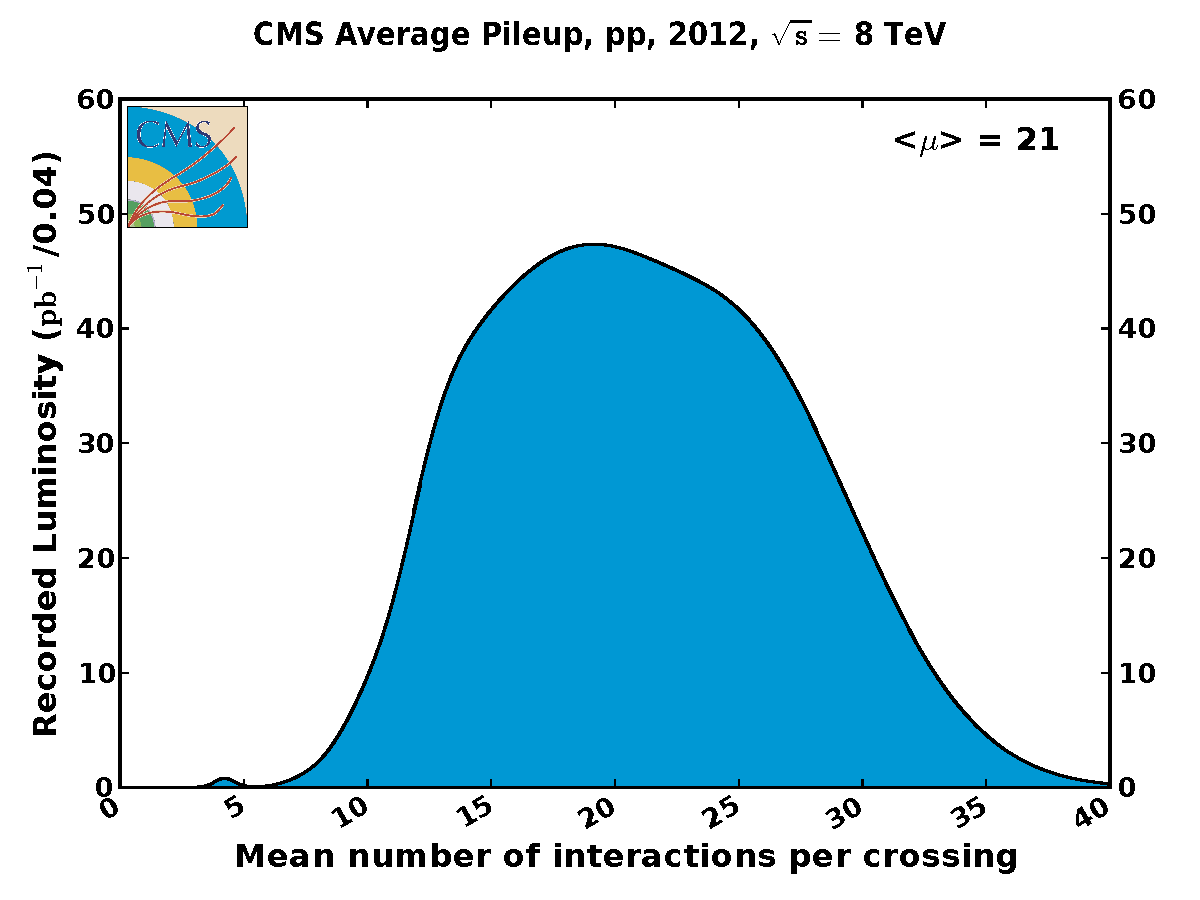
\includegraphics[width=0.7\textwidth]{plots/detector/pileup_pp_2012-2.pdf}
\caption[Distribution of number of pileup events per bunch crossing in 2012
data.]{Distribution of number of pileup events per bunch crossing in 2012 data \cite{cmslumitwiki}.}
\label{fig:PU}
\end{figure}

\section{The CMS experiment}
\label{sec:CMSInDetail}

The CMS detector is a general purpose detector designed to search for the
\ac{SM} Higgs and new physics. As discussed in section~\ref{sec:SMHiggs}, the
mass of the Higgs boson is not directly predicted by the \ac{SM}, and hence upon
design it was important that CMS be able to achieve sensitivity to the \ac{SM} Higgs for a
wide range of possible masses. As shown in figure~\ref{fig:SMHiggsBRs}, at different
Higgs masses the branching ratios of the Higgs boson to different final states
vary considerably, and so CMS must be able to detect the particles from a wide
range of possible decay channels. Thus CMS is a hermetic detector featuring
a layered system of different subdetectors, each of importance to the detection
of different particles. 

\begin{figure}[htbp]
   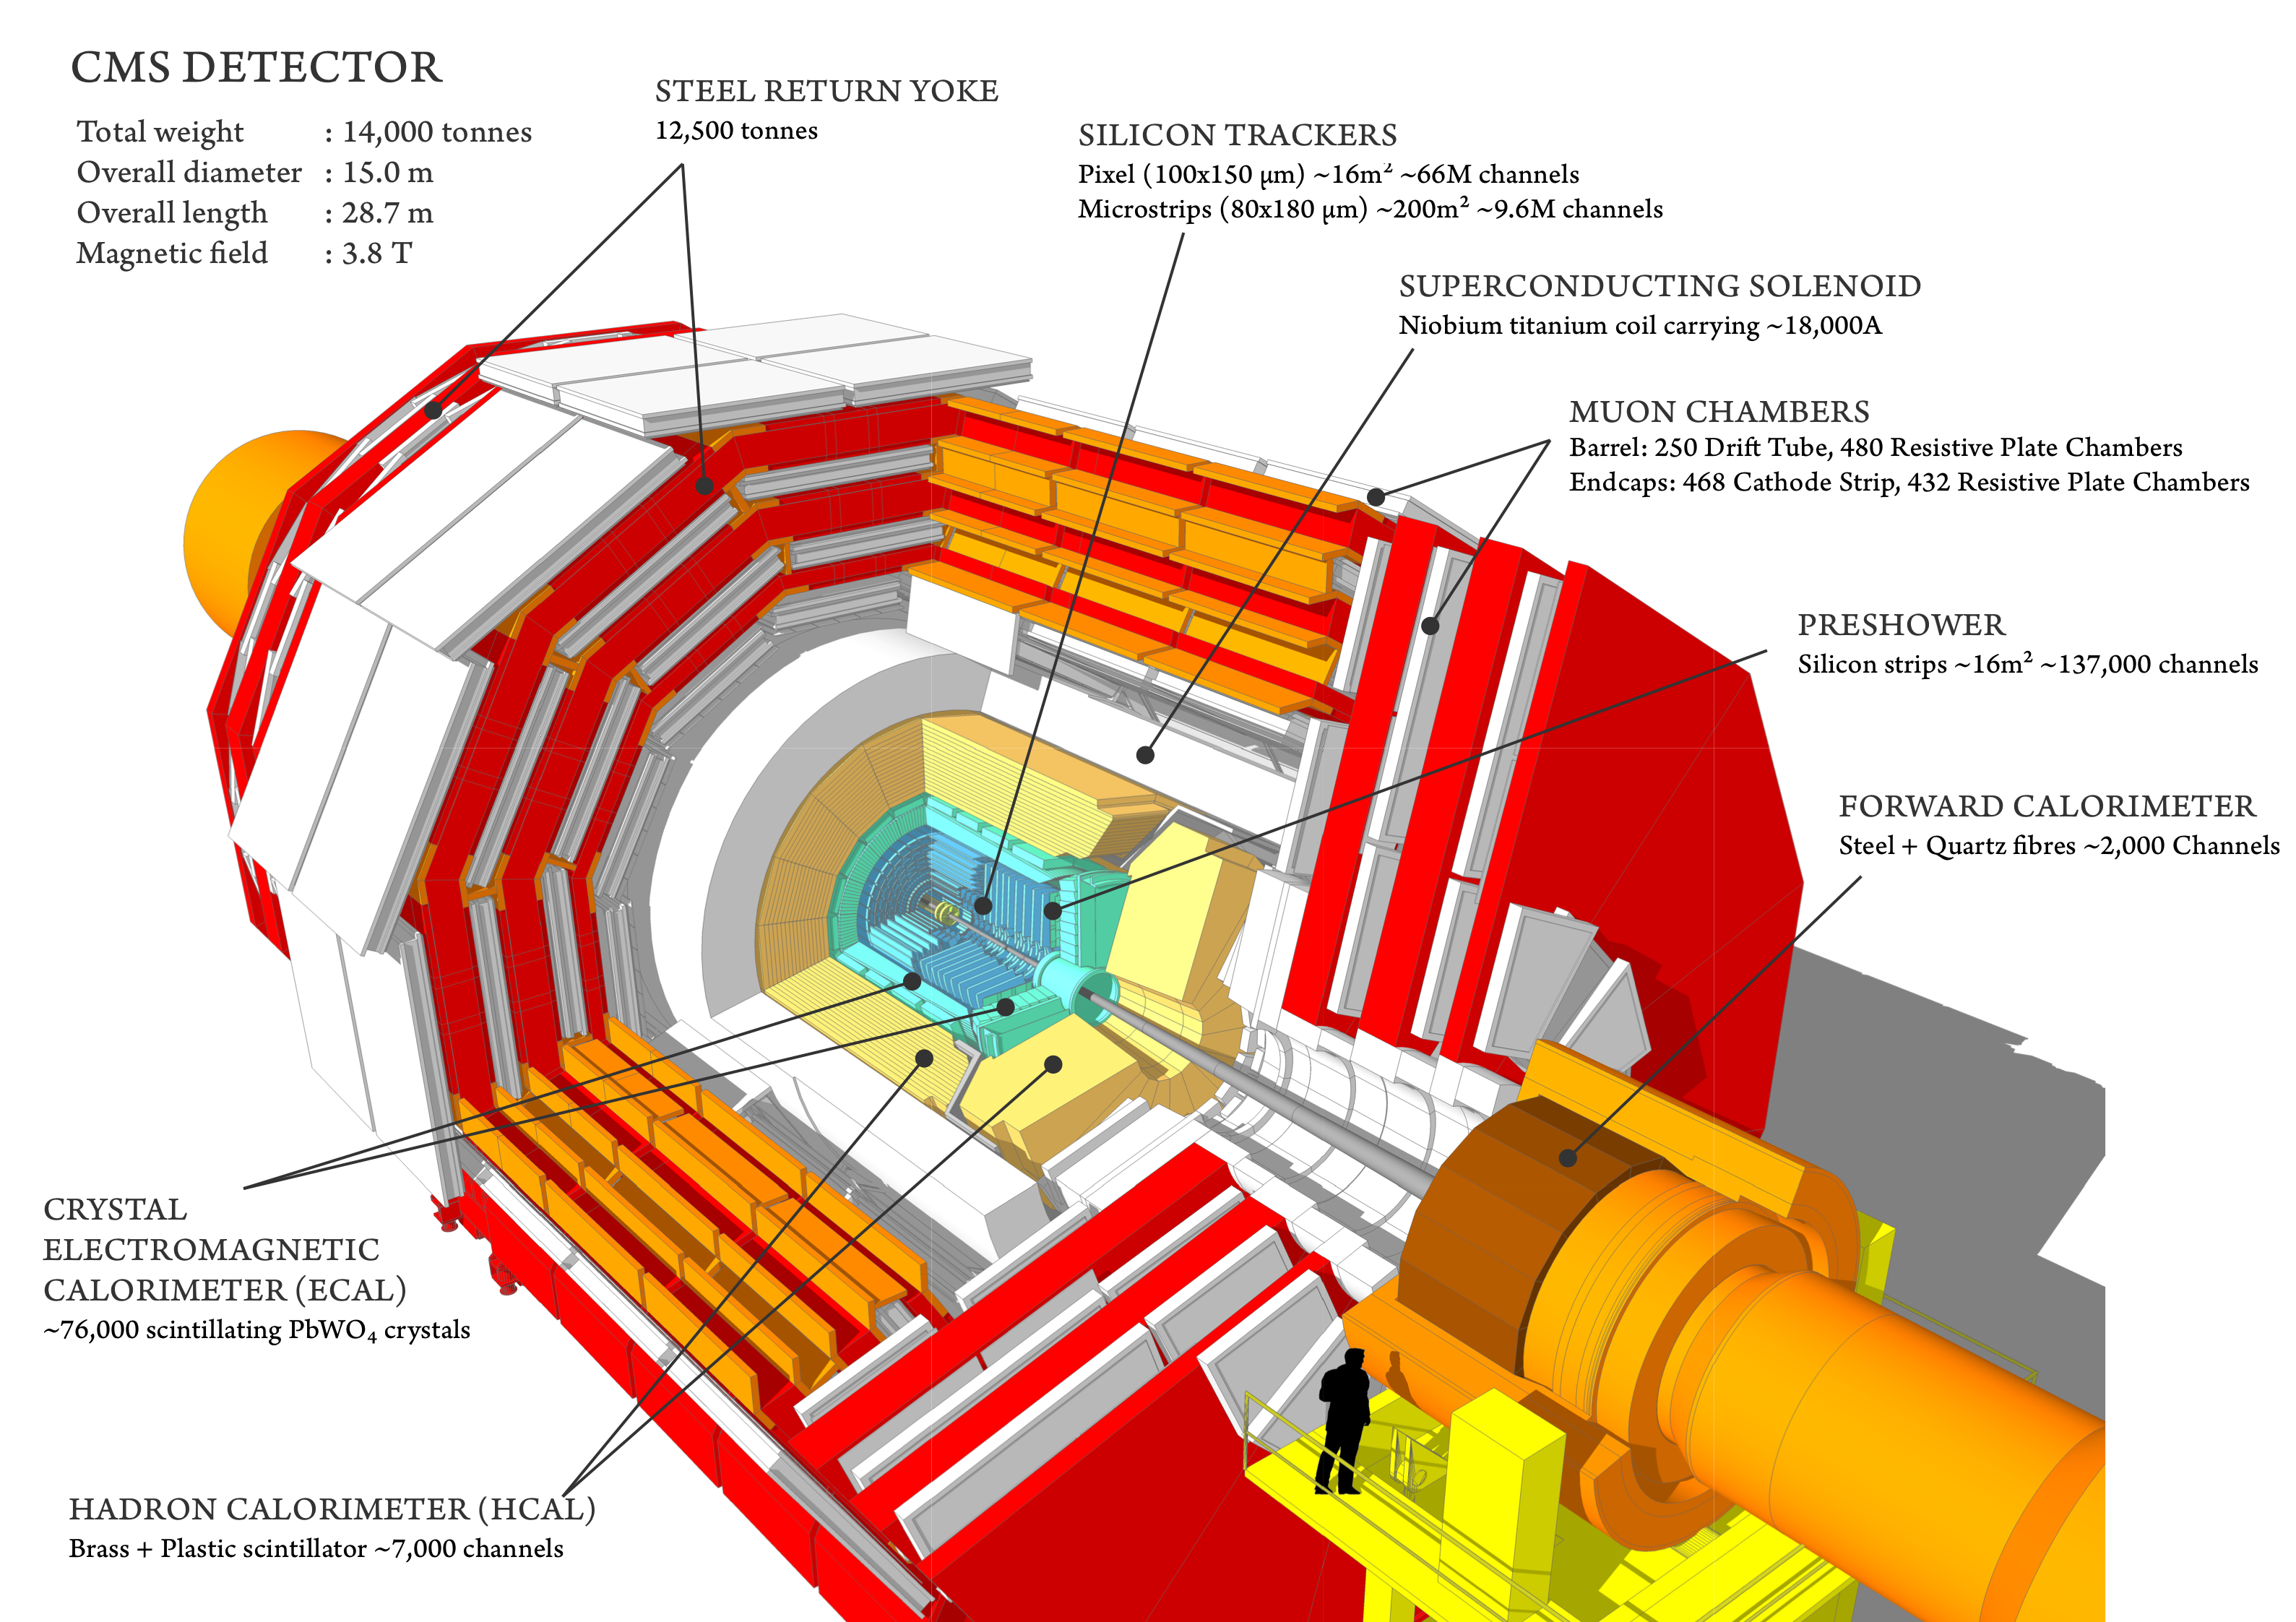
\includegraphics[width=0.95\textwidth]{plots/detector/CMS_Schematic.png}
\caption[A schematic of the CMS detector, illustrating the positions of the
various subdetectors.]
{A schematic of the CMS detector, illustrating the positions of the
various subdetectors~\cite{1742-6596-513-2-022032}.}
\label{fig:CMSschematic}
\end{figure}

A schematic of the CMS detector is shown in figure~\ref{fig:CMSschematic}. 
The first layer is the tracker, which records the tracks of charged particles,
from which can be extracted the particle's momentum and the location of the
vertex from which it originated. This is followed by the \ac{ECAL} which measures
energy deposited in electromagnetic showers from electrons or photons. The
\ac{HCAL} does a similar job for the hadronic activity, by providing energy
measurements of collections of hadrons, known as jets, which deposit energy
through nuclear interactions. The \ac{HCAL} is a sampling calorimeter, meaning
that the active material is sandwiched between dense absorbing material to
increase the depth of the calorimeter to around 11 interaction lengths. The
\ac{HCAL} coverage is increased in the forward regions by the adinteraction 
the \ac{HF} calorimeter. The tracker and calorimeters are encased within a 3.8T axial magnetic
field provided by a superconducting magnet which forms the next layer. This
magnetic field provides the mechanism for deflecting the charged particle paths in
a curve such that their momentum can be measured by the size of the curve in the
track and their charge by the direction. The
outermost layers form the muon detector systems, interspersed with iron plates
of the return yoke of the magnet. Muons deposit little energy
through the detector and often travel through to the surrounding cavern. 
%The entire CMS detector is $22\,\metre$ long and $15\,\metre$ in diameter
%\cite{Chatrchyan:2008aa}.

CMS uses a right handed cartesian coordinate system. The
origin is placed at the nominal interaction point with the $z$ axis collinear with the
beam. Then the $x$ axis is chosen to point towards the centre of the LHC ring
and forms a plane with $y$, the remaining transverse coordinate perpendicular to
$x$ and $z$ in the upwards direction. The angle $\phi$ is the azimuthal angle with respect to the $x$
axis and $\theta$ is the polar angle in the $x$--$y$ plane. The coordinate $r$
is used for the radial coordinate when describing CMS in terms of a cylindrical
coordinate system. Another coordinate often used is pseudorapidity, defined as:
\begin{equation}
\eta = - \ln[\tan(\theta/2)]. 
\end{equation}

Distance in the $\eta$-$\phi$ plane is given by $\Delta R =
\sqrt{\Delta\phi^{2} + \Delta\eta^{2}}$.
Another important quantity relating to the measurement of collisions is the
projection of the momentum of a particle onto the transverse plane: $\pt =
\sqrt{p_{x}^{2} + p_{y}^{2}}$. The corresponding transverse energy is referred
to as $E_{\text T}$. Hard collisions generally produce particles with
high $\pt$. Descriptions of the detector often separate the regions of
``barrel'' and ``endcaps'', which correspond to the main cylindrical body of
the detector or the circular ends enclosing the cylinder respectively. 

%Figure~\ref{fig:CMSslice} shows a slice of the CMS detector, illustrating 
%the paths of various particles through the different subdetectors.

%\begin{figure}[htbp]
%   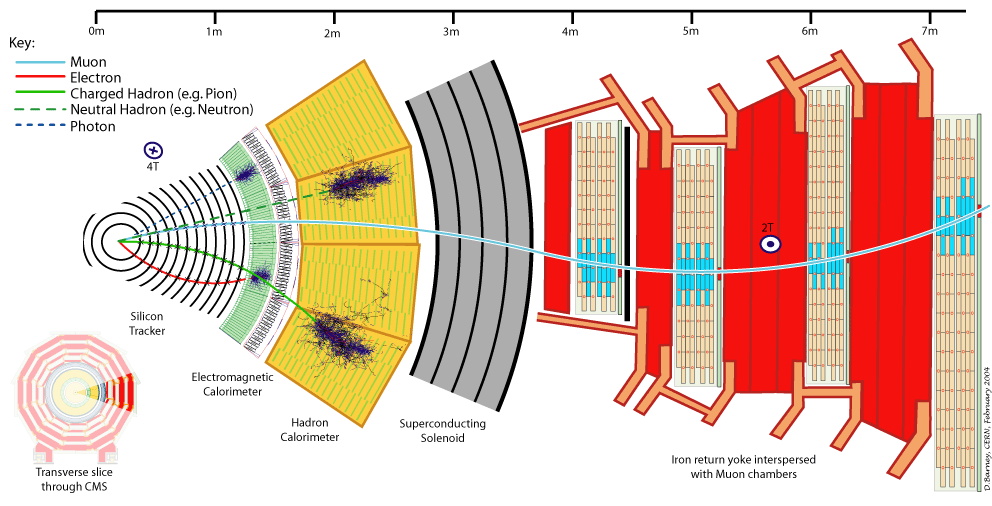
\includegraphics[width=0.9\textwidth]{plots/detector/CMS_Slice.png}
%\caption[A slice of the CMS detector, indicating the various subdetectors.]
%{A slice of the CMS detector, indicating the various subdetectors. The
%paths taken by different types of particles travelling through the detector are
%indicated.}
%\label{fig:CMSslice}
%\end{figure}

\subsection{Tracker}
\label{sec:tracker}

The CMS tracker is designed to reconstruct charged particles close to the
interaction point \cite{Chatrchyan:2008aa}. The magnetic field in combination with the tracker allows
measurement of the particle's momentum and charge. This requires a high level of
granularity to make precise measurements of positions of particles and hence to
locate the vertex from which they originate. Due to the design bunch spacing
of the LHC of $25~\ns$, the rate of collision is extremely high, and so the tracker is
required to be both fast response and radiation hard. This motivates the use of a
silicon based tracking system.

The layout of the tracker is shown in figure~\ref{fig:trackerlayout}.
The tracker is composed of layers of silicon pixel and strip detectors covering
the pseudorapidity range $|\eta| < 2.5$. The pixel detector consists of 66
million individual silicon pixels, each $100~\micron \times 150~\micron$
in size, forming three layers in the barrel region and two in each endcap. The
spatial resolution of the pixel detector is $10$ and $20\micron$ in the $r$--$\phi$ plane
and the $z$ direction respectively, allowing a three-dimensional vertex reconstruction.
Surrounding the pixel detector are layers of strip detectors. These consist of
four cylindrical layers which extend to $r=55\,\cm$ referred to as the
\ac{TIB}, and three disks in each endcap referred to as the \ac{TID}. Each strip
is $10$--$20\,\cm$ long and $80$--$180\,\micron$ wide. Surrounding the \ac{TIB}
and \ac{TID} is the \ac{TOB}, which extends to $r=116\,\cm$ and
$z=\pm118\,\cm$ and contains six barrel layers. The \ac{TEC} comprises nine
disks covering the endcaps. The position resolution of the strip detectors is in
the range $23$--$52\,\micron$ in the $r$--$\phi$ plane and $230$--$530\,\micron$
in the $z$ direction depending on layer. Better resolution in the $r$--$\phi$
plane is required for the measurement of $\pt$.

\begin{figure}[htbp]
   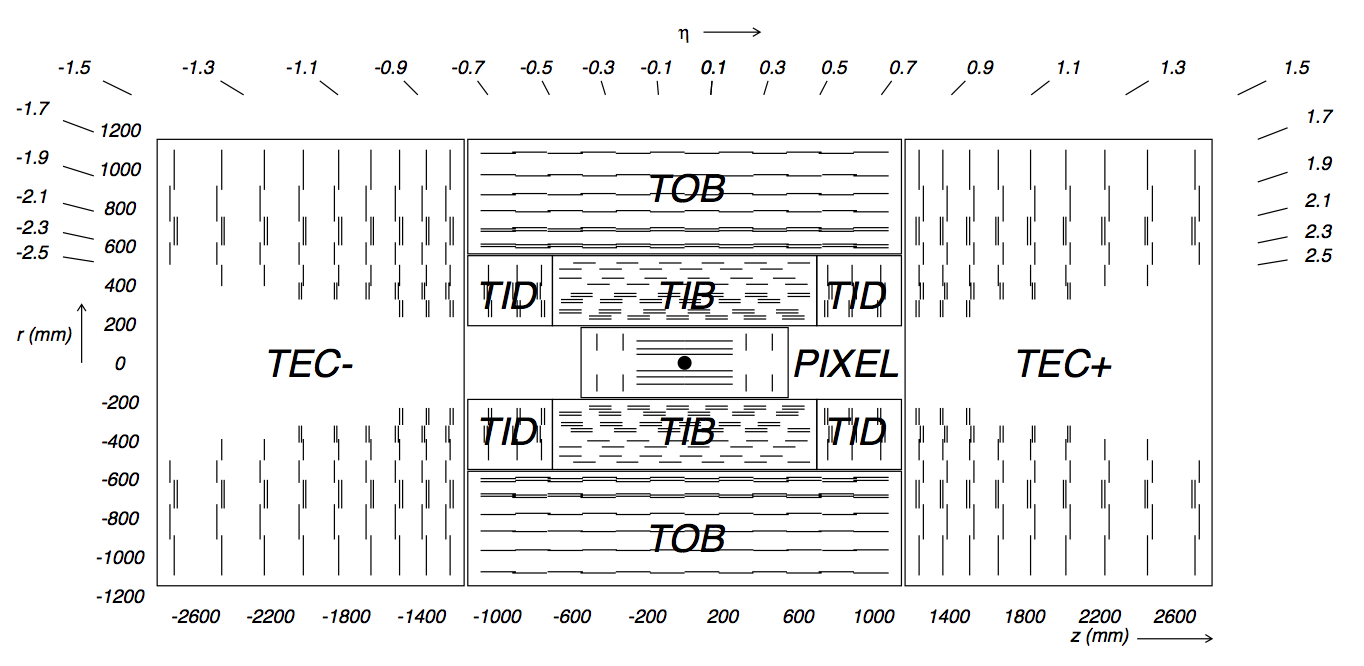
\includegraphics[width=0.9\textwidth]{plots/detector/tracker_layout.png}
\caption[Cross-section of the CMS tracking system, indicating the pixel and
strip detectors and their positions relative to the interaction point.]
{Cross-section of the CMS tracking system, indicating the pixel and
strip detectors and their positions relative to the interaction point \cite{Chatrchyan:2008aa}.}
\label{fig:trackerlayout}
\end{figure}

Tracks are reconstructed using multiple precise measurements throughout the
tracking system. The reconstruction is seeded by triplets of hits in the inner
tracking layers. The trajectory of this seed is extrapolated to the outer tracking
layers using the Kalman filter method \cite{Fruhwirth:1987fm}. The hits found in each layer
which are compatible are added to the trajectory and its uncertainties are
updated until no more compatible hits are found. The use of the tracks to
reconstruct the \ac{PV} is discussed further in section \ref{sec:vertex}.
Momentum resolution degrades with increasing momentum due to decreasing
curvature in the tracks. The $\pt$ resolution of muon tracks is approximately
$1$--$2\%$ for muons with $\pt$ as high as $100\,\GeV$ in the region
$|\eta|<1.6$, rising as high as $8\%$ in the larger $\eta$ regions which have
lower coverage~\cite{Chatrchyan:2008aa}.  

\subsection{Electromagnetic calorimeter}
\label{sec:ecal}

The \ac{ECAL} is constructed from high density lead tungstate
($\mathrm{PbWO_{4}}$) crystals which form a barrel section (EB) 
and two endcaps (EE) outside the tracker~\cite{Chatrchyan:2008aa}. 
$\mathrm{PbWO_{4}}$ was chosen for its
radiation hardness, short radiation length ($0.89\,\cm$) and small Moli\`ere
radius ($2.2\,\cm$), meaning that almost the entire photon or electron energy
can be deposited in the \ac{ECAL}. High energy electrons or photons
entering a crystal initiate an electromagnetic shower, which produces a cascade
of low energy electrons and photons which undergo bremsstrahlung and pair
production respectively. The shower will continue until energy falls below pair
production threshold and ionisation begins to dominate for electrons. 
The depth of each crystal is equivalent to 25.8 radiation lengths, and
thus electrons and photons deposit most of their energy within the crystals.
The atoms in the $\mathrm{PbWO_{4}}$ de-excite by producing scintillation light that is read by
photodetectors. The decay time of the scintillation light is short, such that
about 80\% is emitted before the next bunch crossing (within $25\,\ns$). This
results in a calorimeter with excellent energy resolution, granularity and timing
precision.

Figure \ref{fig:ecal} shows the layout of the \ac{ECAL}. The EB covers the
pseudorapidity range $|\eta|<1.479$. The crystals are arranged in 36 modules such
that the gap between modules are offset by $3^\circ$ with respect to the axis
from the detector origin to avoid particles travelling along the gaps between
crystals. In
the endcaps the crystals are arranged in an $x$--$y$ grid each with an area of
28.6$\,\times\,$28.6 $\mathrm{mm^{2}}$. Two lead plates and two silicon strip
layers mounted before the EE form the pre-shower detectors (PS). These correspond to about
three radiation lengths of absorber material and are designed to initiate
showering and provide sufficient resolution to distinguish single photons from
the pairs produced in neutral pion decays. Uninstrumented regions exist
between the EB and EE, $1.442 < |\eta| < 1.566$, through which cables pass. It
is not possible to provide good measurement of electrons and photons traversing
this region. Overall the \ac{ECAL} covers a pseudorapidity range of $|\eta|<3$.

\begin{figure}[htbp]
   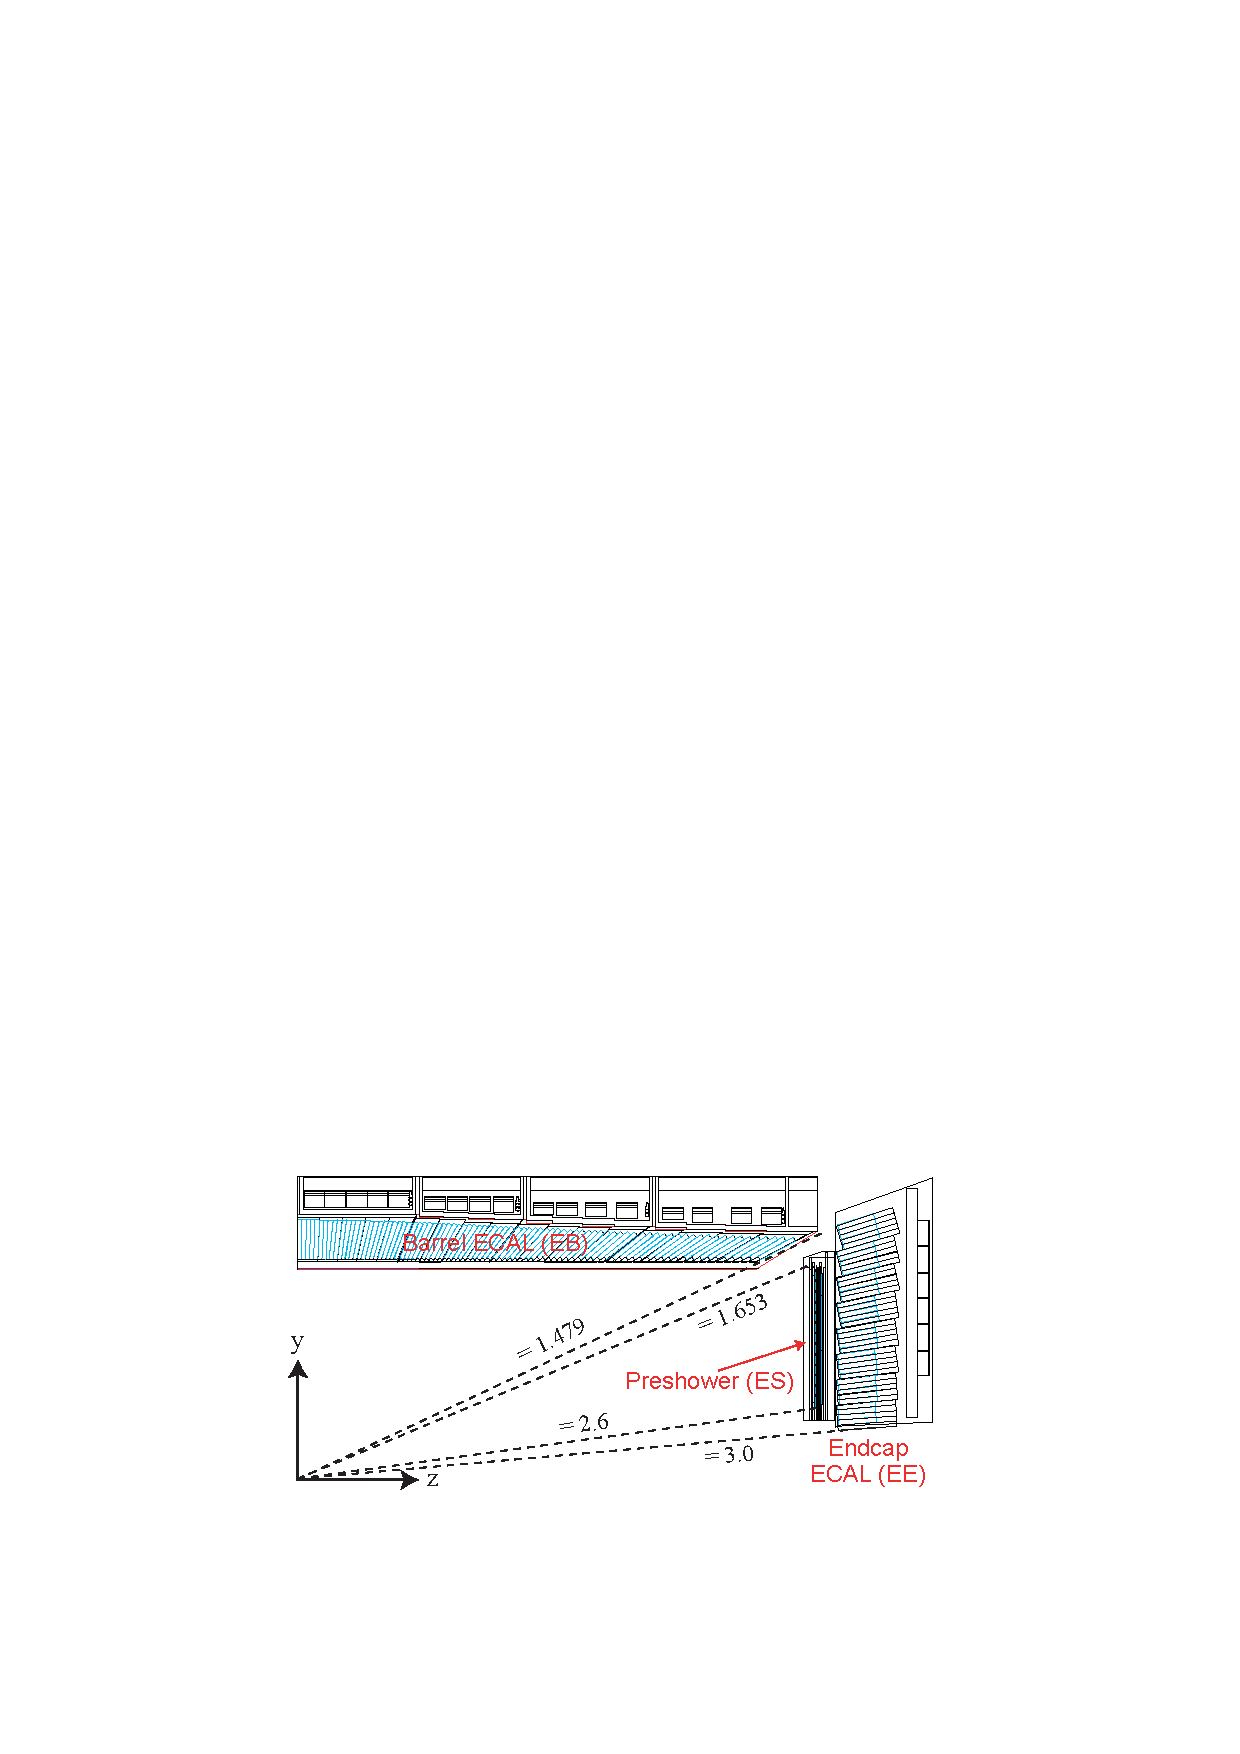
\includegraphics[width=0.9\textwidth]{plots/detector/ecal_layout.pdf}
\caption[Transverse section through the ECAL, indicating its geometry.]
{Transverse section through the \ac{ECAL}, indicating its geometry. The
parts of the detector in the barrel (EB) and endcaps (EE) are indicated
\cite{TDR}.}
\label{fig:ecal}
\end{figure}

The energy resolution of the \ac{ECAL} can be parametrised as a combination of
three unrelated uncertainties as follows:

\begin{equation}
\frac{\sigma}{E} = \frac{A}{\sqrt{E}} \oplus \frac{B}{E} \oplus C , 
\end{equation}

where $E$ is the energy of the incident particle in $\GeV$ and $A$, $B$ and $C$ are the
stochastic, noise and constant contributions respectively. The constants are
derived from test beam data \cite{Chatrchyan:2008aa}. The stochastic term, ($A=2.83\pm0.3\%$),
parametrises stochastic fluctuations in scintillation and shower shape, and is
very low for lead tungstate since the shower can mostly be contained within the
crystals. The noise term $B=0.12\,\GeV$ is determined by the electronics. The
constant term $C=0.26\pm0.4\%$ accounts for non uniformity of read-out, 
and limits the \ac{ECAL} accuracy at high energies.
High resolution is essential to allow accurate reconstruction of high energy
photons, such as those produced in $\PH\to\Pphoton\Pphoton$ decays, an important
discovery channel for the \ac{SM} Higgs.

\subsection{Hadronic calorimeter}
\label{sec:hcal}

The sampling \ac{HCAL} surrounds the \ac{ECAL} and also
covers the pseudorapidity range $|\eta|<3$~\cite{Chatrchyan:2008aa}. The
\ac{HCAL} is designed to detect and measure the energy of strongly interacting
particles. It consists of alternating layers of brass absorber and plastic
scintillator. Brass is used as the absorber material due to its fairly short
nuclear interaction length ($16.42\,\cm$) and the fact that it is not magnetic
\cite{PDG}. A hadron shower initiated in an absorber layer causes pulses of 
light in the plastic scintillator tiles which are fed to hybrid photodiodes 
by wavelength shifting fibres. Surrounding the \ac{HCAL} is the solenoid magnet,
the additional material of which maximises shower containment and reduces 
non-Gaussian tails in energy resolution due to energy loss. 

The layout of the \ac{HCAL} is shown in figure \ref{fig:hcal}. The \ac{HB}
covers $|\eta|<1.4$ and is read out in towers of size
$\Delta\eta \times \Delta\phi = 0.087\times0.087$. The \ac{HO}
is a layer of scintillating tiles lining the outside of the solenoid, and
samples the tails of the highly penetrating or late starting showers using the magnet coil as an
absorber. The \ac{HE} at each end of the barrel
consist of towers with dimensions varying between $\Delta\eta \times \Delta\phi
= 0.087\times0.8$ and $0.35\times0.8$. The \ac{HB} provides between 5.8 and 10.6
interaction lengths of absorber, and in combination with the \ac{HO} this increases
to a minimum of $11.8$ interaction lengths. The \ac{HE} provides approximately
10 interaction lengths. 

The \ac{HF} detectors extend the \ac{HCAL} to cover up
to $|\eta|=5.2$ and experience the highest fluxes of particles in the whole
detector, and so are made using radiation hard quartz fibres as the active medium
embedded in a steel absorber. In the \ac{HF} a signal is generated when charged
showering hadrons emit Cherenkov radiation in the fibre, which is detected by
photomultiplier tubes. The \ac{HCAL} contains no
uninstrumented regions. The large coverage of the
\ac{HCAL} is necessary to be able to accurately calculate the missing transverse energy
(\MET) in an event as a result of neutrinos which are invisible to the detector,
using energy balance with the visible objects. This is discussed further in
section~\ref{sec:met}.


\begin{figure}[htbp]
   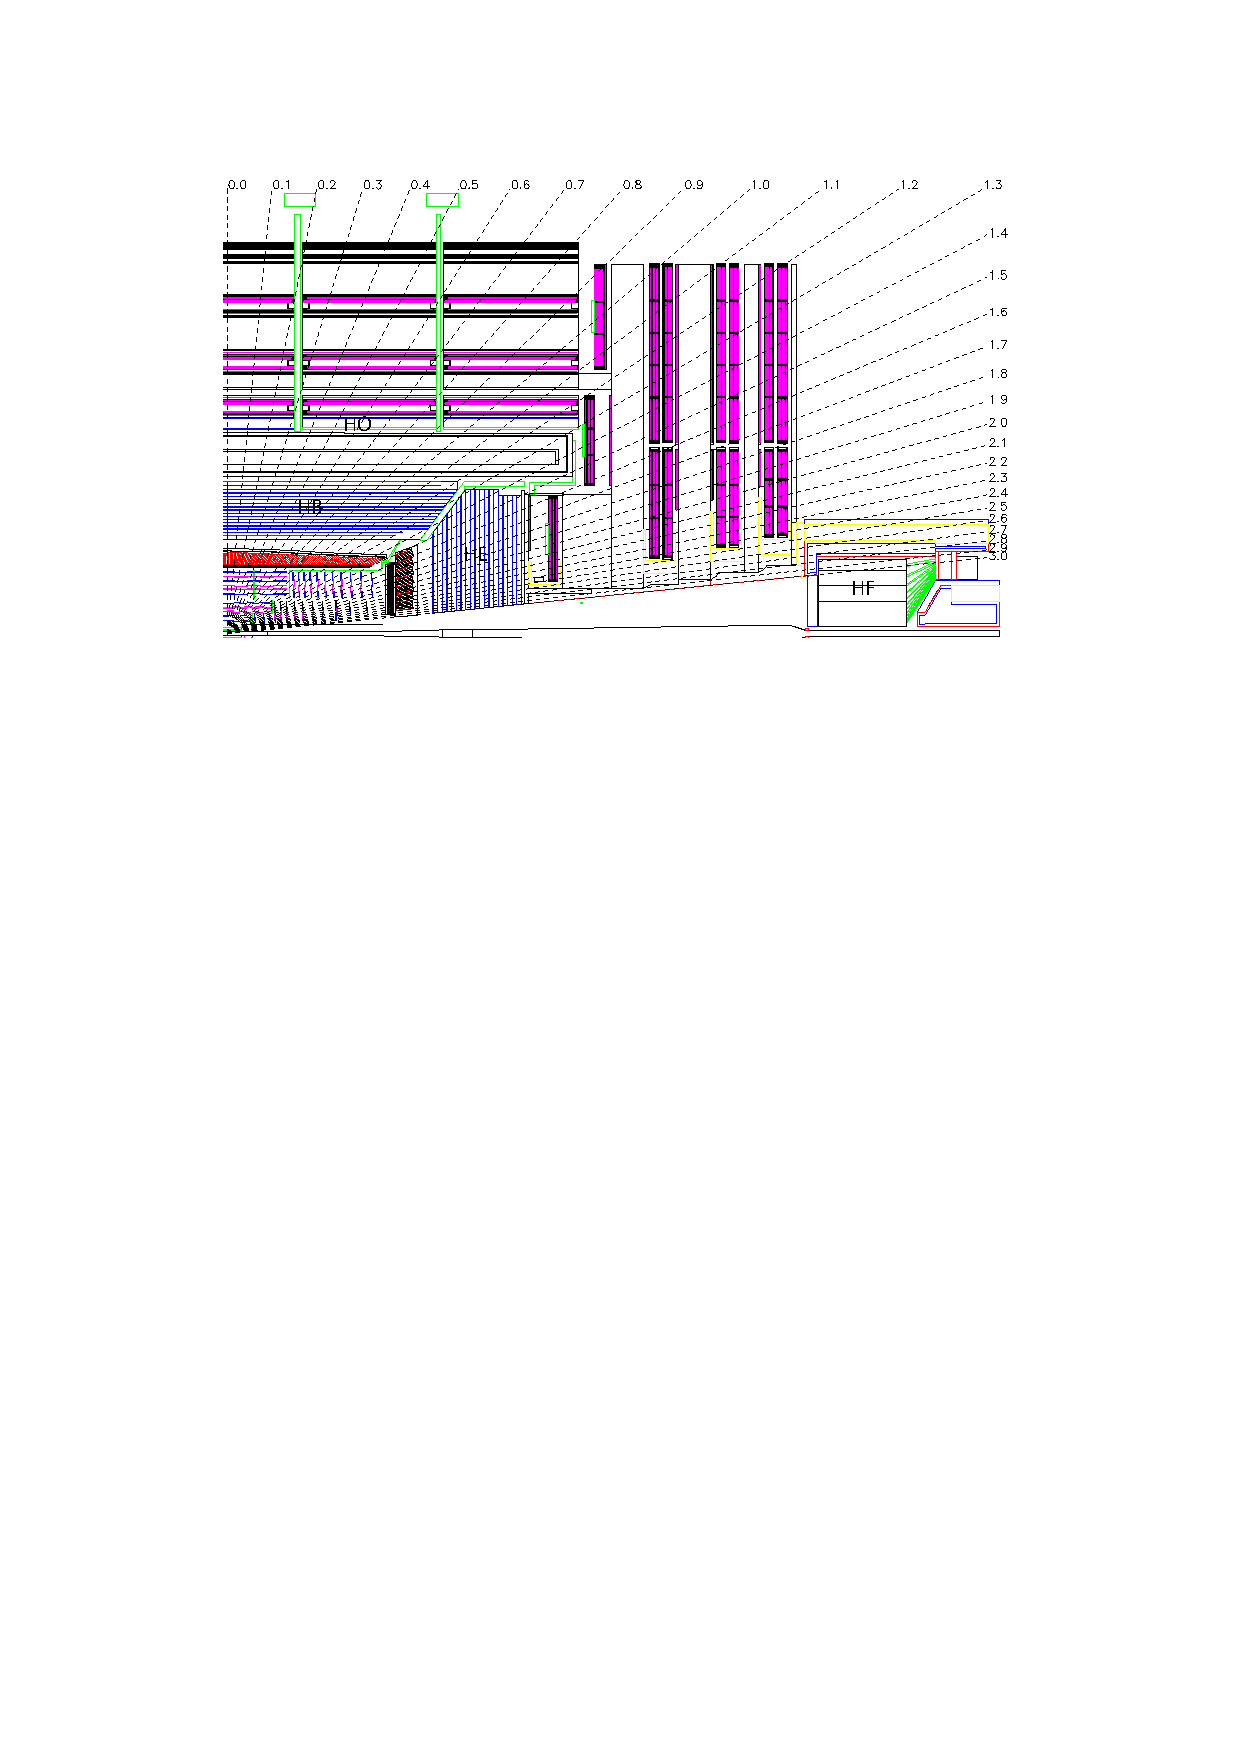
\includegraphics[width=0.9\textwidth]{plots/detector/hcal_layout.pdf}
\caption[Illustration of the HCAL in the r--z plane, indicating its
geometry.]
{Illustration of the \ac{HCAL} in the r--z plane, indicating its geometry \cite{Chatrchyan:2008aa}.}
\label{fig:hcal}
\end{figure}

Both the granularity and the energy resolution of the \ac{HCAL} are worse than
the \ac{ECAL}. The resolution is measured using a test beam of charged pions and
found to be \cite{Abdullin:2009zz}:

\begin{equation}
\frac{\sigma}{E} = \frac{94.3\%}{\sqrt{E}} \oplus 8.4\%,
\end{equation}

where $E$ is the energy of the showering particle. 

\subsection{Muon detector}
\label{sec:muondetector}

The iron return flux of the magnet is instrumented with the muon detectors
\cite{Chatrchyan:2008aa}, covering a pseudorapidity range of $|\eta|<2.4$. Due
to the fact that muons have considerably higher masses than electrons, they lose
little energy via bremsstrahlung or ionisation, and so typically pass through
the calorimeters and the solenoid without depositing much energy. The muon
systems are therefore used for efficient identification of muons, as well as
being able to provide a complementary measurement of their momentum additional
to the one made in the tracker. The best momentum resolution is achieved by 
combining hits in the tracker and the muon chambers, as described in section~\ref{sec:muons}. 

The muon detector is shown in figure \ref{fig:muondetectors}. The barrel region
(covering $|\eta|<1.2$) consists of the \ac{DT} chambers arranged in four
cylindrical layers positioned between the plates of the magnet return yoke. The
\ac{DT}s are augmented by \ac{RPC} in the range covering $|\eta|<1.6$. The
\ac{DT} chambers consist of a tube of cross section $13\times42\,\text{mm}^{2}$,
each filled with wires about $2.4\,\metre$ long. The tubes are filled with a
mixture of argon and carbon dioxide gas. When a muon travels through the tube,
it ionises the gas, and free electrons drift towards the anode wire resulting in
an electrical signal. Each chamber consists of several layers of tubes, oriented
in different directions to measure the muon $\phi$ direction and the $z$
coordinate. The position resolution of the \ac{DT}s is approximately
$200~\micron$.

\begin{figure}[htbp]
   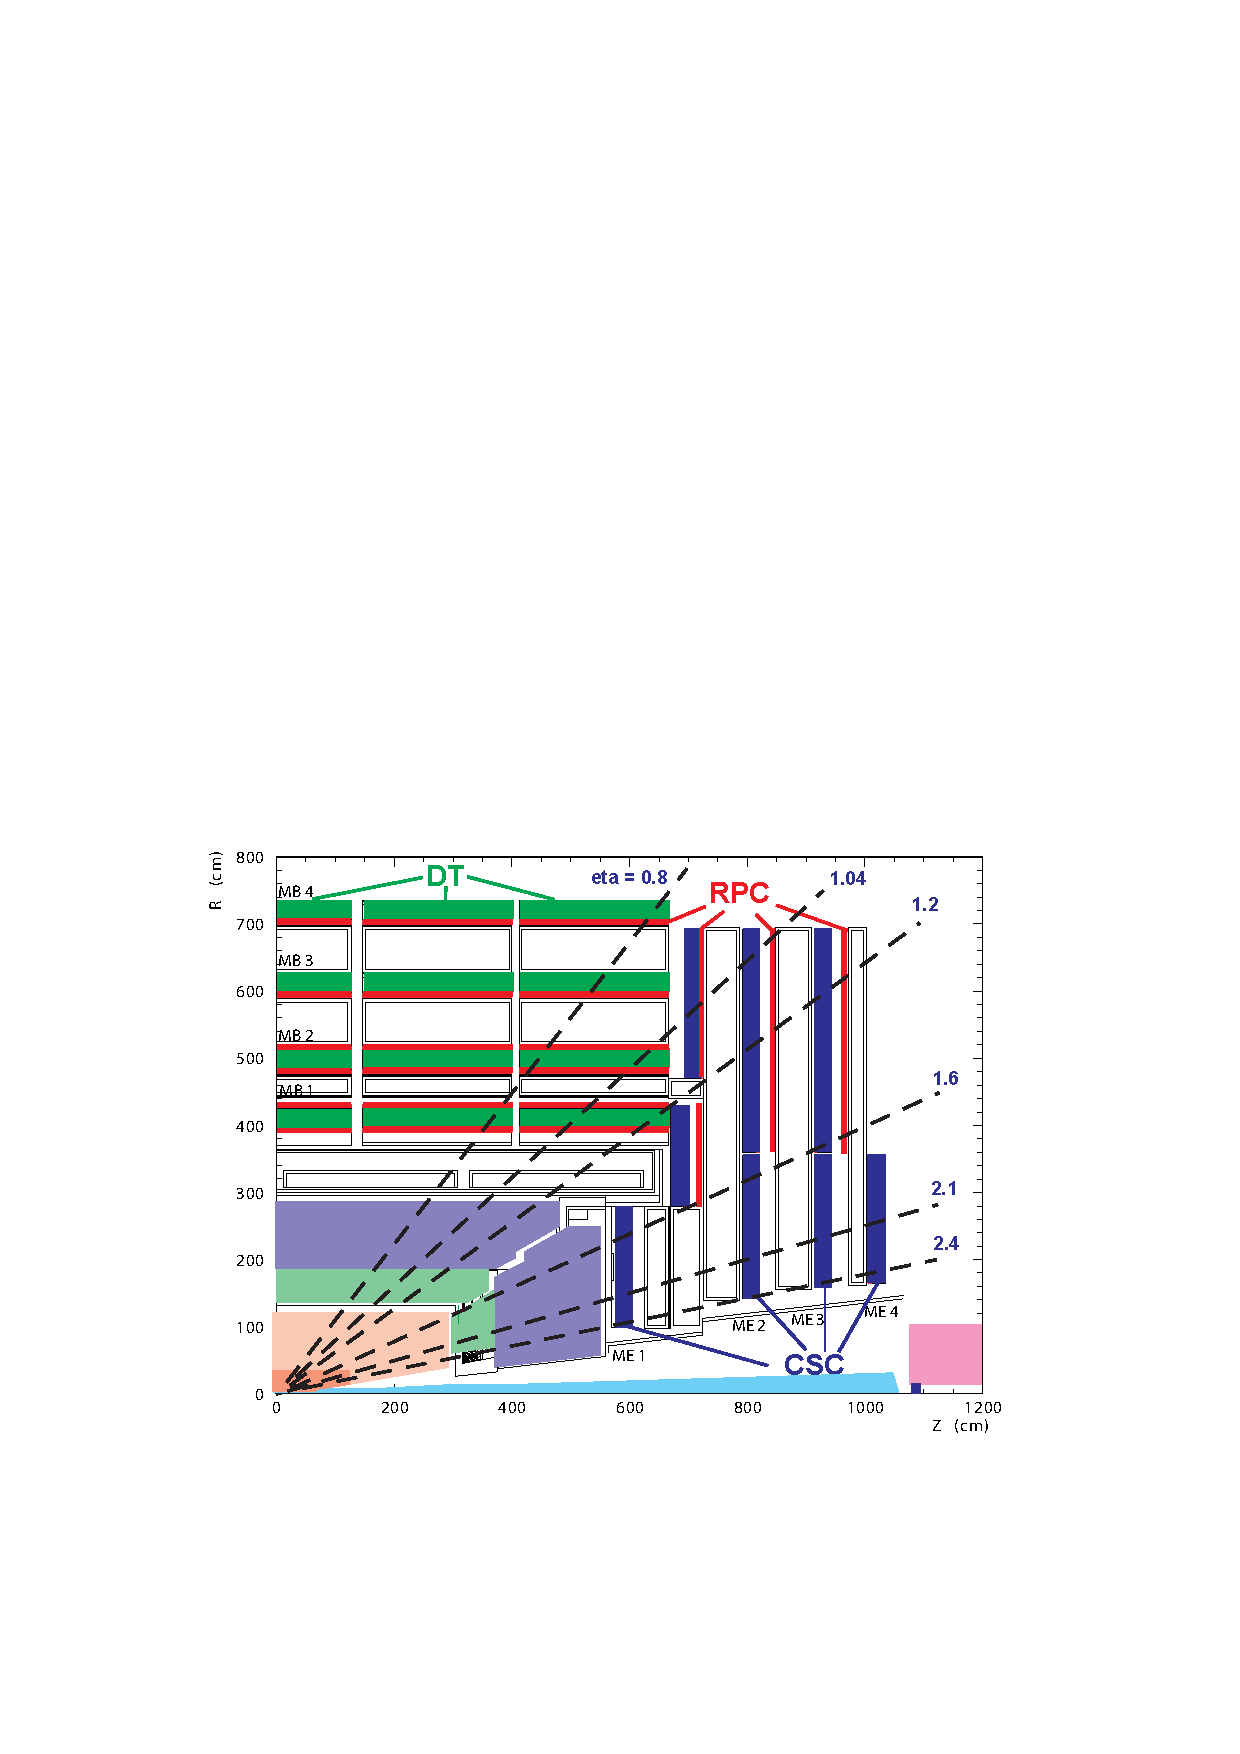
\includegraphics[width=0.9\textwidth]{plots/detector/muon_layout.pdf}
\caption[Layout of one quadrant of the muon systems.]{
    Layout of one quadrant of the muon systems, indicating the positions
of the DT, CSC and RPC \cite{TDR}.}
\label{fig:muondetectors}
\end{figure}

The endcaps use \ac{CSC}s, which have a fast response, fine segmentation and are
radiation hard. This is necessary in the endcaps due to the higher rate of muons
and backgrounds from soft neutrons. Each \ac{CSC} has six gas layers with cathode strips running
radially outward to measure hits in the $r$-$\phi$ plane, with anode wires
running perpendicular to the cathodes to measure $\eta$. The position resolution
of the \ac{CSC}s varies between 100 and $200~\micron$ depending on $\eta$. In the region
$|\eta|<1.6$, the \ac{CSC}s are augmented by \ac{RPC}s, as in the barrel. The
\ac{RPC}s consist of a gas gap enclosed by parallel anode and cathode plates, in
which the muon ionisation is detected by arrays of metallic strips running
parallel to the beam axis. The \ac{RPC}s have worse resolution than the \ac{DT}s
and \ac{CSC}s but an extremely fast time response of
$1~\ns$, meaning they can be used to correctly identify the bunch crossing in
which a muon originates, and can be used as a dedicated muon trigger.


\subsection{Triggering and data processing}
\label{sec:trigger}

At the design specification of the LHC, the proton bunch crossing rate is
$40~\MHz$, and to date collisions have been recorded at $20~\MHz$, which will
increase to the design $40~\MHz$ in Run 2 starting this year. Each event
consists of approximately $1~\text{MB}$ of data and it is not feasible to write
data at this rate to tape, nor is it feasible for the \ac{DAQ} system to perform
read-out of the events at this rate. Thus the rate at which events are saved is
reduced to $\mathcal{O}(1\,\kHz)$ using a trigger system to select the
interesting events.

The first stage of the trigger system is the \ac{L1} trigger, which is
constructed using custom electronics to incorporate information from the
calorimeters and muon systems only~\cite{Chatrchyan:2008aa}. The \ac{L1} starts with local information
such as calorimeter energy deposits and hit patterns in the muon chambers. A
regional trigger combines this local trigger information from different sections
of the detector to give a $\pt$ sorted list of candidate objects. Finally the
global trigger issues a decision to accept or reject the event based on the
\ac{L1} information from all parts of the detector. This decision is made within
$3.2\,\micro\second$ and uses only the front-end electronics. The \ac{L1}
trigger reduces the rate to around $100\,\kHz$.  

Events accepted by the \ac{L1} trigger are then read out to the \ac{HLT}. This
operates on a processor farm of several thousand CPU cores and processes the 
complete detector information, including input from the tracker. The \ac{HLT}
is capable of determining the object momenta with much greater accuracy, and
apply tighter identification criteria, using algorithms much closer to those
used in offline reconstruction. Due to the fact that the instantaneous luminosity
increased across the Run 1 period, the trigger $\pt$ and energy thresholds were
changed several times in order to retain a stable rate of read-out. Over the Run
1 period, CMS operated at a rate of about $1\,\kHz$, with $300\,\Hz$ being promptly
reconstructed and the rest being ``parked'' to be reconstructed after the LHC running
finished when more computing power was freed \cite{CMS:2012ooa}.

Even incorporating the trigger, the rate of production of data by CMS is at
several petabytes per year. The CMS and the other LHC experiments make use of
the \ac{WLCG} \cite{web:grid}, a global data storage and analysis network which
integrates the computing facilities of universities and research institutes
around the world. The system consists of different tiers: the Tier~0 centre at
CERN performs full event reconstruction, before all data are distributed to at
least one Tier~1 centre, to keep a copy at several sites across the globe. A
larger number of Tier~2 centres process these data for specific analyses to give
access to researchers across the globe. 
